\documentclass[a4paper]{article}

\usepackage[english]{babel}
\usepackage[utf8]{inputenc}
\usepackage{amsmath}
%\usepackage[colorinlistoftodos]{todonotes}
\usepackage{amsmath}
\usepackage{listings}
\usepackage{color}
\usepackage{hyperref}
\usepackage{graphicx}
\graphicspath{{../pics/}}

\lstset{frame=tb,
  language=Matlab,
  aboveskip=3mm,
  belowskip=3mm,
  showstringspaces=false,
  columns=flexible,
  basicstyle={\small\ttfamily},
  numbers=left,
  numberstyle=\tiny\color{gray},
  keywordstyle=\color{blue},
  commentstyle=\color{green},
  stringstyle=\color{red},
  breaklines=true,
  breakatwhitespace=true,   
  tabsize=4
}

\title{Machine Learning (course 1DT071)
Uppsala University – Spring 2015
Report for Assignment 1 by group 6}

\author{Ludvig Sundstr\"{o}m and John Shaw}
\date{\today}

\begin{document}

\maketitle

\section{Task1}

For the first task we were asked to create a feed forward neural network (NN) and 
train it to implement the boolean XOR function. Using tools built into Matlab, we 
could experiment with different networks and observe the training process. 
We don't know how the trained neural network finds its solution, 
but in order to understand how to train the network we somehow need to 
visualize the training process. 
Using gradient descent training, we can think of the training process for each problem 
as finding the lowest point in a landscape. If there exists a global minimum point in 
this landscape, we want the training algorithm to find it. There can exist local minima 
though and we don't want the algorithm to get stuck in one, so we want to 
adjust the parameters of the descent in such a way that we don't get stuck in a local 
minimum. After a session of trial and error, we found that a learning rate of 2 
usually resulted in a well-trained network. 

%Insert training plots here
\begin{figure}[h!] %float here
	\caption{\label{fig:plot2_LR2}TODO: Running some examples}
	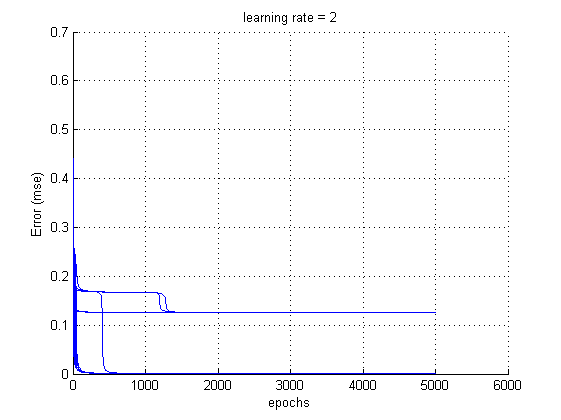
\includegraphics[]{plot2_LR2.png}
\end{figure}
\subsection*{Question 1\& 2}
\textbf{Question 1 \& 2} Sometimes, as shown in for example figure \ref{fig:plot2_LR2}, 
the error plot converges to an value significally larger than zero.
This is because the error rate is too low and we get stuck in local minima. We are 
taking too small steps, and can't get out of small cavities. A too large learning 
rate however, will cause the algorithm to take giant leaps through the landscape. 
Too big steps will make it very hard to find a good solution, and an oscillating 
behaviour is likely to occur; see figure 3. 

%insert colored xor plot 
A visualisation of a well trained network for the xor problem  
is to plot the result of various values 
as colors (figure 4). 
Here, we can see the classification of the possible input values. We can 
clearly see the two hyperplanes generated that seperates data. 

Here, we also see the hidden node values of possible inputs of the XOR function.
Inspecting the plot ranges of the hidden nodes aswell as the output node, we notice that
the range for the hidden nodes are [-1, 1] and the range for the output function is [0, 1].
\textbf{Question 3} The reason that the ranges differs is that two 
different sigmoid functions were used as activation functions used for the network. 
For the hidden layer, the hyberbolic tangent function (range [-1, 1]) were used. 
For the output node, the logistic function (range [0, 1]) were used. The authors of 
this report could not find out weather it makes a difference for the algorithm weather 
you use a activation function that ranges from [0, 1] or [-1, 1] but it's obviously 
convinient if the output activation function has the same range as the actual problem 
output. \textbf{Question 4}A new neural network gets distrubited random weights 
when initialized. The result of this is that the training ends with different 
solutions every time the network is initialized and trained and the 
number of epochs needed to train the network differs aswell. 
\textbf{Question 5} Again consider the colored plot of the XOR problem 
network nodes (figure 4). We already 
know that this represents a well trained network which means that the output node is 
infact representing the boolean XOR function. As for the hidden nodes, study the value 
of the different inputs. For hidden node 1, an input of (0, 0) corresponds to 0 (or 
atleast a value very close to zero). $(0, 1)$ also yeilds $~ 0$, $(1, 0) ~= 0$ and 
$(1, 1) ~= 1$. If this node implemented any boolean function it would be the AND function.
In the same way, the hidden node implements the boolean OR function. 
\textbf{Question 6} This is veryfied in the truth table below. 

\begin{center}
    \begin{tabular} {l | c | r }
        Input & boolean XOR & Network implemented XOR \\
        0 0 & 0 & TODO \\
        0 1 & 1 & TODO \\
        1 0 & 1 & TODO \\
        1 1 & 0 & TODO \\
    \end{tabular}
\end{center}

\section{Task2}
\section{Task3}
\section{Task4}
\section{Appendix}

%code goes below (if needed)
\begin{lstlisting}
\end{lstlisting}

\begin{thebibliography}{9}
	\bibitem{textbook}
		T.H Cormen, C. E. Leiserson, R. L. Rivest, C. Stein 	
				\textit{Introduction to Algorithms}, 3rd edition 2009, p. 708-722, 658-659 \\
	\bibitem{dijkstra}
		\url{http://en.wikipedia.org/wiki/Dijkstra's\_algorithm} \\
	\bibitem{priqueue}
		\url{http://en.wikipedia.org/wiki/Priority\_queue} \\
	\bibitem{bipartite}
		\url{http://www.geeksforgeeks.org/bipartite-graph/}
	\bibitem{bfs}
		\url{http://www.personal.kent.edu/~rmuhamma/Algorithms/MyAlgorithms/GraphAlgor/breadthSearch.htm}
\end{thebibliography}

Ideas, and general pointers how to solve the various problems have been extracted from these resources. Other then that, we declare that the content of this report is entirely pure, coming purely and directly from the it's authors brains.  

\end{document}
